\documentclass[11pt,twoside]{memoireuqam1.3}
\uqammemoire   %% Pour la page titre d'un m�moire

\usepackage{graphicx}% Pour les figures
\usepackage[french]{babel}
%\usepackage[T1]{fontenc} % pour windows surtout, pas bon
\usepackage[utf8]{inputenc} % Pour utiliser les caract�res accentu�s sous Unix

\usepackage{float}
\usepackage{alltt}
\usepackage{url}
\usepackage{tabularx}
\usepackage[usenames]{color}
\usepackage{fnamed}
\usepackage{lmodern}
%\usepackage[cyr]{aeguill} % old school, d�pass�
\usepackage[font=small]{caption}

\input macros  % Pour les d�finitions personnelles

\floatstyle{boxed}
\restylefloat{figure}

\lstset{ basicstyle=\small,       % the size of the fonts that are used for the code
numbers=left,                   % where to put the line-numbers
numberstyle=\footnotesize,      % the size of the fonts that are used for the line-numbers
numbersep=5pt,                  % how far the line-numbers are from the code
tabsize=4,                      % sets default tabsize to 2 spaces
literate=
       {�}{{\,c}}1
       {�}{{\'e}}1
       {�}{{\`e}}1
       {�}{{\`a}}1
       {�}{{\'E}}1
       {�}{{\`E}}1
       {�}{{\`A}}1
       {`}{{\`{}}}1,
}

\begin{document}

%%%%%%%%%%%%%%%%%%%%
% Pour la page titre
%%%%%%%%%%%%%%%%%%%%

% Le titre ne supporte pas les accent simples
\title{Un m\'emoire UQAMien avec un long titre, une~ligne~non~interropue}
\author{Alexis Laferri\`ere}
\degreemonth{Mars}
\degreeyear{2012}
\uqammemoire
% ou
% \uqamthese   %% Pour la page titre d'une th�se
% ou
% \uqamrapport %% Pour la page titre d'un rapport

% Le d�partement doit �tre modifi� dans memoireuqam1.3.cls

\thispagestyle{empty}        % La page titre n'est pas num�rot�e
\maketitle

%%%%%%%%%%%%%%%%%%%%
% Page pr�liminaires
%%%%%%%%%%%%%%%%%%%%
%\renewcommand \bibname{R\'EF\'ERENCES}% FACULTATIF
%Enlever le commentaire, si vous voulez qu'apparaisse le titre R�F�RENCES
% plut�t que BIBLIOGRAPHIE

\renewcommand \listfigurename{LISTE DES FIGURES}
\renewcommand \appendixname{APPENDICE}
\renewcommand \figurename{Figure}
\renewcommand \tablename{Tableau}

\pagenumbering{roman} % num�rotation des pages en chiffres romains
\addtocounter{page}{1} % Pour que les remerciements commencent � la page ii
\cleardoublepage
\thispagestyle{empty} % pas num�rot�e

   \parskip=0pt
   \vspace*{0.1 truecm} 
   \begin{center}
    {\uppercase { REMERCIEMENTS }}\par
   \end{center}
   \nobreak \vspace*{1.10 truecm}
   \parskip=2ex

Remerciements particuliers à mon directeur de recherche, Jean Privat,  professeur au département d'informatique de l'UQAM, pour tout son aide, sa patience, le partage de sa vision et la réalisation du langage Nit. Je remercie également mes collègues du groupe de recherche, le GRÉSIL, avec qui j'ai eu la chance de collaborer; Jean-Sébastien Gélinas, Alexandre Terrasa, Julien Chevalier, ainsi qu'Étienne Gagnon, directeur du groupe de recherche GRÉSIL et professeur au département d'informatique de l'UQAM.

Je me dois de remercier ma famille et amis qui m'ont supporté au cours de la réalisation de cette étude; Nilo, Shelsy, Arabelle et surtout Christiane ainsi que Sandrine pour leur aide. Sans oublier François et Jodi qui ont malheureusement tout tenté pour m'aider, je vous en suis redevable.

Merci au mot \textit{langage} pour son apparition à 620 reprises dans ce document, spécialement pour sa complicité avec ma coordination pour qu'il soit toujours écrit sous la forme de \textit{lagnage}.

\tableofcontents % Pour g�n�rer la table des mati�res
\listoffigures % Pour g�n�rer la liste des figures
%\listoftables % Pour g�n�rer la liste des tableaux
\include{textes/lexique}
{\abstract

% en gros; contenu du document, originalité, valeur scientifique
% environ 300 mots

% contenu:
% but, nature et envergure de la recherche
% sujets traités
% hypothèses de travail et méthodes utilisées
% principaux résultats
% conclusion auquels ont est arrivé

% 4 ou 5 mots clés

L'interface native permet à un logiciel de profiter des avantages des langages natifs ainsi que de ceux du langage de haut niveau. Elle intervient entre les différents langages pour permettre les appels de méthodes et la conversion des données. Son utilisation amène cependant généralement une perte de sûreté à l'exécution du logiciel et son emploi est souvent complexe. 

%FIXME JEAN: à partir d'ici tu ne devrais parler que de Nit et C

Dans le cadre de cette recherche, nous développons l'interface native du langage de programmation à objets Nit. Notre recherche vise à résoudre au mieux les problèmes soulevés par l'utilisation d'une interface native, et ce, par une analyse rigoureuse des différents détails de conception d'une interface. Notre intention est donc de concevoir, selon des objectifs précis, l'interface native idéale pour le langage Nit. Pour mettre à l'épreuve notre proposition, nous avons conçu et implémenté l'interface native du compilateur Nit.

La conception de cette interface native s'appuie donc sur des objectifs que nous considérons garants d'une interface native de qualité. Ces objectifs consistent à préserver la sûreté d'exécution du logiciel, maintenir une connaissance du flot d'appels, utiliser le langage Nit de façon expressive et selon ses forces, conserver une syntaxe naturelle en C ainsi qu'offrir une interface native versatile et d'utilisation rapide par tout autre moyen.

Pour atteindre ces objectifs, nous proposons quatre grandes approches clés; la forme des modules hybrides pour gérer la coexistence de deux langages; une déclaration explicite des appels de méthodes réalisées depuis le langage C pour conserver la connaissance du flot d'appels; une représentation symétrique des types et méthodes Nit en C pour en permettre une utilisation naturelle et vérifiée statiquement; les classes natives qui représentent les types C en Nit et leur appliquent les forces du paradigme de programmation à objets, dont le polymorphisme.

Enfin, pour valider l'interface native proposée et implémentée, nous présentons comment nous avons utilisé cette interface pour réaliser des modules et des logiciels Nit. Nous démontrons également que cette interface peut être utilisée dans le développement d'autres interfaces spécialisées en fonction de besoins spécifiques.

Mots clés: interface native, interface de fonctions étrangères, compilation, langages de programmation à objets
}


% Utilisez l'environnement  abstract pour r�diger votre r�sum�

%%%%%%%%%%%%%%%%%%%%
% Document principal
%%%%%%%%%%%%%%%%%%%%

\parindent=0ex % Facultatif
% pour qu'il n'y ait pas  de renfoncement � chaque alin�a

% Utilisez l'environnement  introduction pour r�diger votre introduction
\include{Introduction}

% contenu:
% sujet et sa portée
% état de la question et problème a resoudre
% objectifs
% méthode utilisée
% démarche adoptée
% structure du document

\begin{introduction}
\label{introduction}

Les langages de programmation de haut niveau, tel que Java~\cite{java}, Python~\cite{pythonRef}, Ruby~\cite{rubyCookbook}, C\#~\cite{csharp} et beaucoup d'autres, sont loin du fonctionnement de la machine physique, simple d'utilisation et offrent aux programmeurs plusieurs services tels qu'un paradigme de programmation avancé, une syntaxe expressive, une gestion automatique de la mémoire ou encore, une assurance de sûreté d'exécution. Le langage de programmation à objets Nit~\cite{nit} est de cette catégorie, il utilise une syntaxe simple, comporte un ramasse-miettes et offre des optimisations statiques à la compilation. En comparaison, le langage C~\cite{ansi-c89} conserve de forts avantages, il permet la programmation près de la machine et l'accès à une grande quantité de code préexistant. 

\section{Langage de programmation Nit}

Nous avons réalisé cette étude dans le cadre du développement du langage de programmation Nit~\cite{nit}. Dans cette section, nous présentons les particularités du langage Nit principalement en rapport avec les autres langages de programmation à objets. Ces particularités sont utiles pour comprendre les décisions que nous avons prises au cours de l'étude et nous leur faisons référence à répétition dans ce document.

\end{introduction}

\chapter{Classes natives}

À l'utilisation de l'interface native, le programmeur doit fréquemment conserver une référence à un espace mémoire ou une donnée C dans le code Nit. Traditionnellement, dans les autres interfaces, cet espace mémoire est opaque au langage de haut niveau et il y est représenté par un type général.


\section{Représentation des types C en Nit}

La figure~\ref{fig:hybride} présente quelque chose.


\begin{figure}[t]
\begin{center}
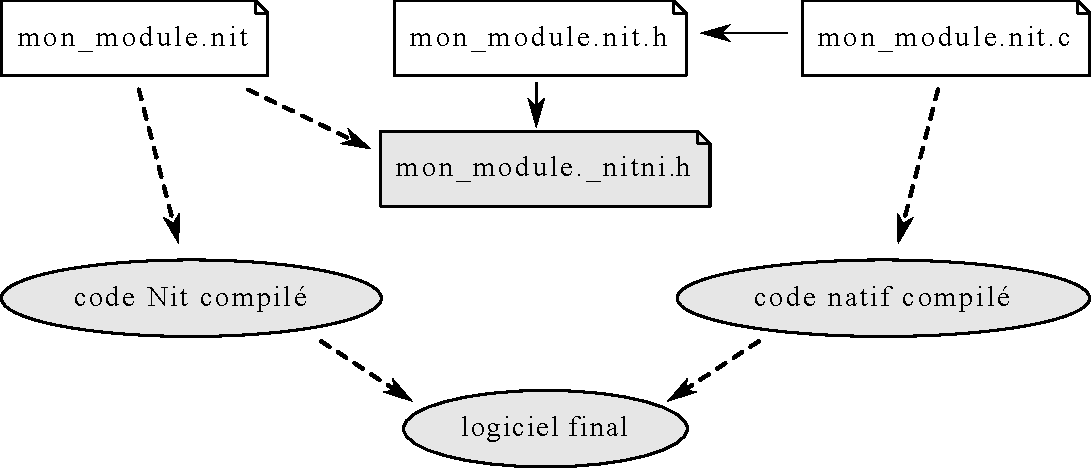
\includegraphics[width=4in]{figures/hybride}

\caption[Short name for the list of figures]{Real caption: Structure of JNI residing between the JVM and the native code.

The JNI is the interface for all JVM functionalities accessible from C. It exposes enough internals of the JVM offering a wide range of uses.}
\label{fig:hybride}
\end{center}
\end{figure}


% Utilisez l'environnement  conclusion pour r�diger votre conclusion
\begin{conclusion}

Dans cette étude, nous traitons le sujet de l'interface native du langage de programmation à objets Nit en ayant pour but de concevoir une interface native idéale pour ce langage. Tout logiciel complexe, tel que ceux comportant une interface graphique, réalisant des opérations réseau ou utilisant toute autre fonction système, se base sur une interface native directement ou indirectement. L'interface native d'un langage est donc largement utilisée, sa qualité influence directement celle de tout logiciel réalisé en ce langage.

\section*{Travaux futurs}

Le concept de l'interface native du langage Nit peut être adapté pour tout autre langage de programmation à objets. Une interface native semblable pourrait être réalisée pour d'autres langages permettant ainsi de bénéficier d'une syntaxe native naturelle et de la sûreté d'exécution amenée par nos contributions.

\end{conclusion}


%%%%%%%%%%%%%%%%%%%%
% Page liminaires
%%%%%%%%%%%%%%%%%%%%

\bibliographystyle{theseuqam2} % non compatible avec le package natbib
\bibliography{biblio-locale}

\end{document}
